\def\QRCODE{TB_IPR_TUT.IMG.binary_morphological_reconstruction_matlabqrcode.png}
\def\QRPAGE{http://www.iptutorials.science/tree/master/TB_IPR/TUT.IMG.binary_morphological_reconstruction/matlab}

\mcorrectionsection{Matlab correction}

Images given as examples are stored as binary images. The structuring elements used, square, line and disk, are defined with the \matlabregistered{} function \minline{strel}, and some parameters (of size and shape).

\begin{matlab}
% read image 
B=imread('B.bmp');
% display image
figure;imshow(B,[]);title('Original image');

% Create structuring elements
se1 = strel('square',11) ;     % 15-by-15 square
se2 = strel('line',11,45);     % line, length 15, angle 45 degrees
se3 = strel('disk',5);        % disk, radius 15
\end{matlab}

\subsection{Dilation}
The dilation operation is illustrated in Fig.\ref{fig:matlab:morphology_reconstruction:dilation}.

\begin{figure}[htbp]
 \centering
 \subfloat[Square structuring element.]{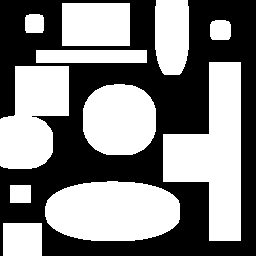
\includegraphics[width=.3\linewidth]{dilate_square.png}}\hfill
 \subfloat[Line structuring element.]{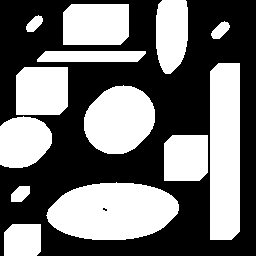
\includegraphics[width=.3\linewidth]{dilate_line.png}}\hfill
 \subfloat[Disk structuring element.]{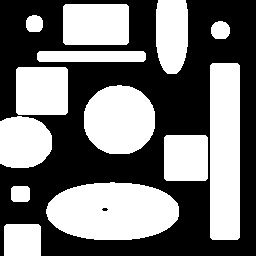
\includegraphics[width=.3\linewidth]{dilate_disk.png}}
 \caption{Dilation with different structuring elements.}
 \label{fig:matlab:morphology_reconstruction:dilation}
\end{figure}
  
\begin{matlab}
figure;
% dilation
dilateSquare = imdilate(B, se1);
dilateLine = imdilate(B, se2);
dilateDisk = imdilate(B, se3);
subplot(4,3,1); imshow(dilateSquare);title('dilation, square');
subplot(4,3,2); imshow(dilateLine);title('dilation, segment');
subplot(4,3,3); imshow(dilateDisk);title('dilation, disk');
\end{matlab}

\subsection{Erosion}The dual operation of dilation is the erosion,illustrated in Fig.\ref{fig:matlab:morphology_reconstruction:erosion}.

\begin{figure}[htbp]
 \centering
 \subfloat[Square structuring element.]{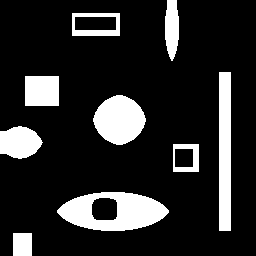
\includegraphics[width=.3\linewidth]{erode_square.png}}\hfill
 \subfloat[Line structuring element.]{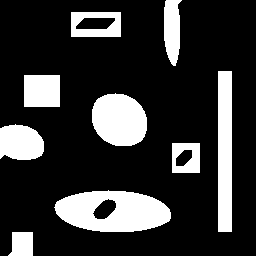
\includegraphics[width=.3\linewidth]{erode_line.png}}\hfill
 \subfloat[Disk structuring element.]{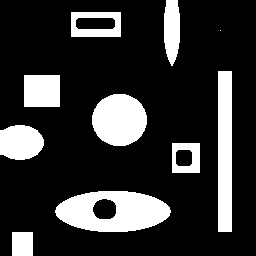
\includegraphics[width=.3\linewidth]{erode_disk.png}}
 \caption{Erosion with different structuring elements.}
 \label{fig:matlab:morphology_reconstruction:erosion}
\end{figure}

\begin{matlab}
% erosion
erodeSquare = imerode(B, se1);
erodeLine = imerode(B, se2);
erodeDisk = imerode(B, se3);
\end{matlab}

\subsection{Opening and closing}
Opening and closing are the combination of erosion and dilation in both orders, see illustration Fig.\ref{fig:matlab:morphology_reconstruction:openclose}.
\begin{matlab}
% open
openSquare = imopen(B, se1);
openLine = imopen(B, se2);
openDisk = imopen(B, se3);
\end{matlab}

\begin{matlab}
% close
closeSquare = imclose(B, se1);
closeLine = imclose(B, se2);
closeDisk = imclose(B, se3);
\end{matlab}


\begin{figure}[htbp]
 \centering
 \subfloat[Opening with a square structuring element.]{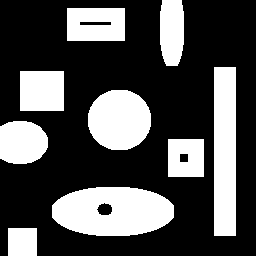
\includegraphics[width=.3\linewidth]{opening_square.png}}\hfill
 \subfloat[Opening with a line structuring element.]{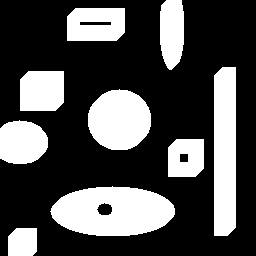
\includegraphics[width=.3\linewidth]{opening_line.png}}\hfill
 \subfloat[Opening with a disk structuring element.]{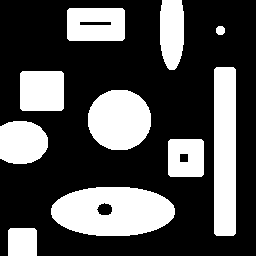
\includegraphics[width=.3\linewidth]{opening_disk.png}}
 
  \subfloat[Closing with a square structuring element.]{
\includegraphics[width=.3\linewidth]{closing_square.png}}\hfill
 \subfloat[Closing with a line structuring element.]{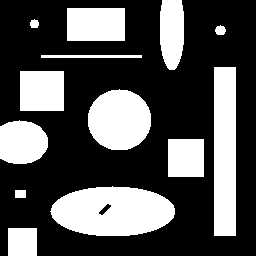
\includegraphics[width=.3\linewidth]{closing_line.png}}\hfill
 \subfloat[Closing with a disk structuring element.]{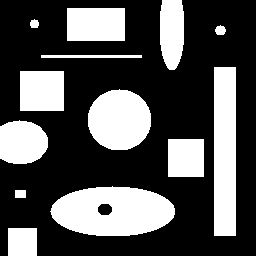
\includegraphics[width=.3\linewidth]{closing_disk.png}}
 \caption{Opening and closing with different structuring elements.}
 \label{fig:matlab:morphology_reconstruction:openclose}
\end{figure}


The following code is used to illustrate the impact of the size of the structuring element.
\begin{matlab}
% 
% opening with varying size
figure;
for i=1:12
    sedisk(i)=strel('disk',i);
    openDisk = imopen(B, sedisk(i));
    subplot(4,3,i); imshow(openDisk);title(strcat('opening, ',int2str(i)));
end
\end{matlab}

\subsection{Morphological reconstruction}
The morphological reconstruction is employed in a lot of applications, like removing objects touching the borders of the image, of removing small objects. The intersection of two sets is coded as the minimum of binary arrays. The result is illustrated in Fig.\ref{fig:matlab:morphology_reconstruction:reconstruction}.

\begin{matlab}
function B=reconstruct(A,M)
M=min(M,A);
r=bwarea(M);
s=0;
se=strel('disk',1);
while (r ~= s)
    s=r;
    M=min(A, imdilate(M, se));
    r=bwarea(M);
end
B=M;
\end{matlab}
 
\begin{figure}[htbp]
\centering
\subfloat[$I_1$]{{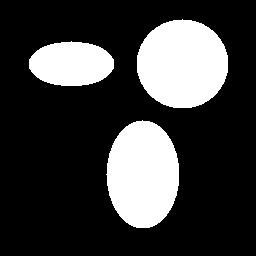
\includegraphics[width=.3\linewidth]{A.png}}}\hspace{.5cm}
\subfloat[$M$]{{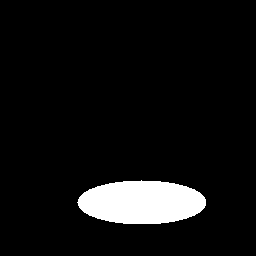
\includegraphics[width=.3\linewidth]{M.png}}}\hspace{.5cm}
\subfloat[$rec(I_1,M)$]{{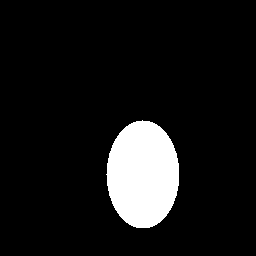
\includegraphics[width=.3\linewidth]{rec.png}}}
\caption{Illustration of morphological reconstruction of $I_1$ by $M$.}
\label{fig:matlab:morphology_reconstruction:reconstruction}
\end{figure}
 
\subsubsection{Remove border objects}
In order to remove the objects that may touch the border, a marker of the border is defined. In practice, the extreme pixels are marked, then the reconstruction of the objects by this marker is performed, then removed from the original image. Notice the definition of a border with value 255, as it can handle unsigned 8 bits images (thanks to the \minline{min} function). See Fig.\ref{fig:matlab:morphology_reconstruction:rec_appli}.
If $\mathcal{B}$ represents the border of the image (create an array of the same size as the image, with zeros everywhere and ones at the sides), then this operation is defined by:
\[ \textrm{killBorders}(I) = I\setminus \rho_I(\mathcal{B})\]

\begin{matlab}
function B=killBorders(A)
[m,n]=size(A);
M=zeros(m,n);
M(1,:)=255;
M(m,:)=255;
M(:,1)=255;
M(:,n)=255;
M=reconstruct(A,M);
B=A-M;
\end{matlab}

\subsubsection{Remove small objects}
The principal is first to make an erosion with a given structuring element $se$, in order to suppress the objects smaller than $se$. Then, a reconstruction is performed in order to get the original objects. See Fig.\ref{fig:matlab:morphology_reconstruction:rec_appli}. 

It consists in an erosion followed by a reconstruction. The structuring element used in the erosion defines the objects considered as ``small''.
\[\textrm{killSmall}(I)=\rho_I(\varepsilon(I)) \]
\begin{matlab}
function B=killSmall(A,n)
se=strel('disk',n);
M=imerode(A,se);
B=reconstruct(A,M);
\end{matlab}

\subsubsection{Close holes}
In order to close holes, we work on the complementary set of $A$ and try to isolate the background (that is supposed to touch the border of the image). See Fig.\ref{fig:matlab:morphology_reconstruction:rec_appli}. The operation is given by the following equation, with $\mathcal{B}$ the border of image $I$, and $X^C$ denoting the complementary of set $X$:
\[ \textrm{removeHoles(I)} = \{ \rho_{I^C}(\mathcal{B})\}^C\]

\begin{matlab}
function B=closeHoles(A)
Ac=imcomplement(A);
[m,n]=size(A);
M=zeros(m,n);
M(1,:)=255;
M(m,:)=255;
M(:,1)=255;
M(:,n)=255;
M=reconstruct(Ac,M);
B=imcomplement(M);
\end{matlab}


\begin{figure}[htbp]
\centering

\subfloat[Close holes in objects.]{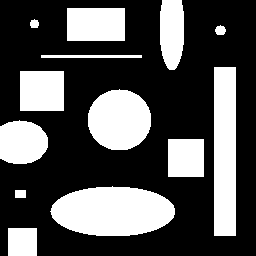
\includegraphics[width=.3\linewidth]{closeholes.png}}\hfill
\subfloat[Kill border objects.]{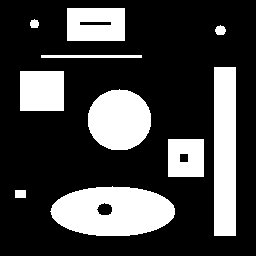
\includegraphics[width=.3\linewidth]{killborders.png}}\hfill
\subfloat[Kill small objects.]{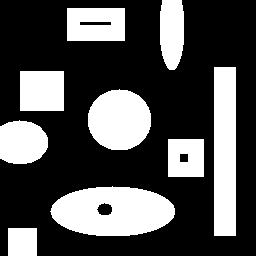
\includegraphics[width=.3\linewidth]{killsmall.png}}
\caption{Illustration of the use of the morphological reconstruction.}
\label{fig:matlab:morphology_reconstruction:rec_appli}
\end{figure}

\subsection{Application on cells image}
The application on the cell image is quite trivial: after thresholding (binarizing) the original image (the threshold value is chosen experimentally), we can close the holes, remove the small objects and the ones touching the borders (see Fig.\ref{fig:matlab:morphology_reconstruction:cells}).

\begin{matlab}
A=imread('cells.bmp');
C=A<98;
B=closeHoles(C);
B=killBorders(B);
B=killSmall(B,5);
\end{matlab}


\begin{figure}[htbp]
\centering

\subfloat[Original image of cells.]{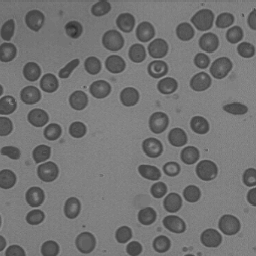
\includegraphics[width=.4\linewidth]{cells.png}}\hfill
\subfloat[Segmented image.]{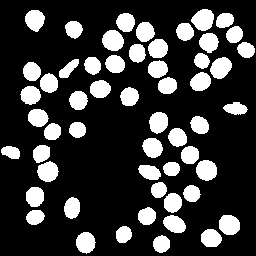
\includegraphics[width=.4\linewidth]{cleancells.png}}
\caption{Segmentation of the image of cells.}
\label{fig:matlab:morphology_reconstruction:cells}
\end{figure}
